% !TEX root = ../thesis.tex
% !TEX spellcheck = en-US

\clearpage

\section{Research process and Design Development}

\subsection{Data}

\todo{Describe data format}

In order to perform supervised learning labelled data was needed for training. Together with the process of reframing of the research problem this was approached in an iterative way. First a quick prototypical tool was built to collect labels in a crowd-sourced fashion. This allowed getting more knowledge about the problem itself, especially with regards to how humans perform the task of labelling topics of text sections, and to perform first experiments of algorithmically achieving meaningful results in agreement to human behavior on this task. Then these learnings were taken into consideration when re-scoping the research problem and according to that data was collected using the microtasking service crowdflower~\cite{crowdflower}, leading to a quality dataset of labelled sentences from job ads.

\subsubsection{Explorative Data Collection}

\todo{Picture of software setup?}

To collect first data a tool was build, consisting of a Node.js~\cite{nodejs} server using MongoDB\cite{mongodb} as a database and communicating via a JSON with a simplistic website front-end using the mustache template engine~\cite{mustache}. The tool is online\footnote{\url{http://thesis.cwestrup.de/jobad-tagger/}} and it's source code is publicly available on GitHub\footnote{\url{https://github.com/cle-ment/thesis-tagger}} with it's API documentation hosted online as well\footnote{\url{http://thesis.cwestrup.de/jobad-tagger/apidoc/}}.

The data generated by using the free text description of each job ad and splitting it into paragraphs as can be seen in the software package as well\footnote{\url{https://github.com/cle-ment/thesis-tagger/blob/master/pre-processing.ipynb}}.

The goal of this prototype tool for data collection was on the one hand to acquire data in order to carry our first experiments as fast as possible, and on the other hand to gain a deeper understanding about the research problem itself by giving an open, unbiased task to the participants. In particular the question at hand was how humans label the content of the different parts of a job ad.

The exact task given to the participants was ``Describe what each section is about by adding one or more tags/keywords to it''. They were shown a job ad that was split into paragraphs and besides each paragraph was a text field to enter 1 or more tags.

\begin{figure}[h]
  \centering
  \includegraphics[width=\textwidth]{img/thesis-tagger-interface.png}
  \caption{Screen capture of the interface of the tagging tool}
\label{fig:thesis-tagger-interface}
\end{figure}

In a first step the tool was only shown to 3 participants to get immediate feedback if the user interface had flaws and whether the task was understood.   Based on this feedback the tool was improved by providing an example for the participants and then tested with a slightly larger group of 12 persons. After correcting a few minor details in the user interface a public link was then shared via social media and other channels with as many people as possible. A few days later the tool was then also shared internally within Sanoma where it was set up as a competition to tag the most possible job ads.

In total 91 job ads were tagged, resulting in 379 tagged text sections and 358 tags.

\todo{Describe data: Different characteristics}
\todo{show distribution?}
\todo{show embedding visualizations}

\begin{figure}[h]
    \centering
    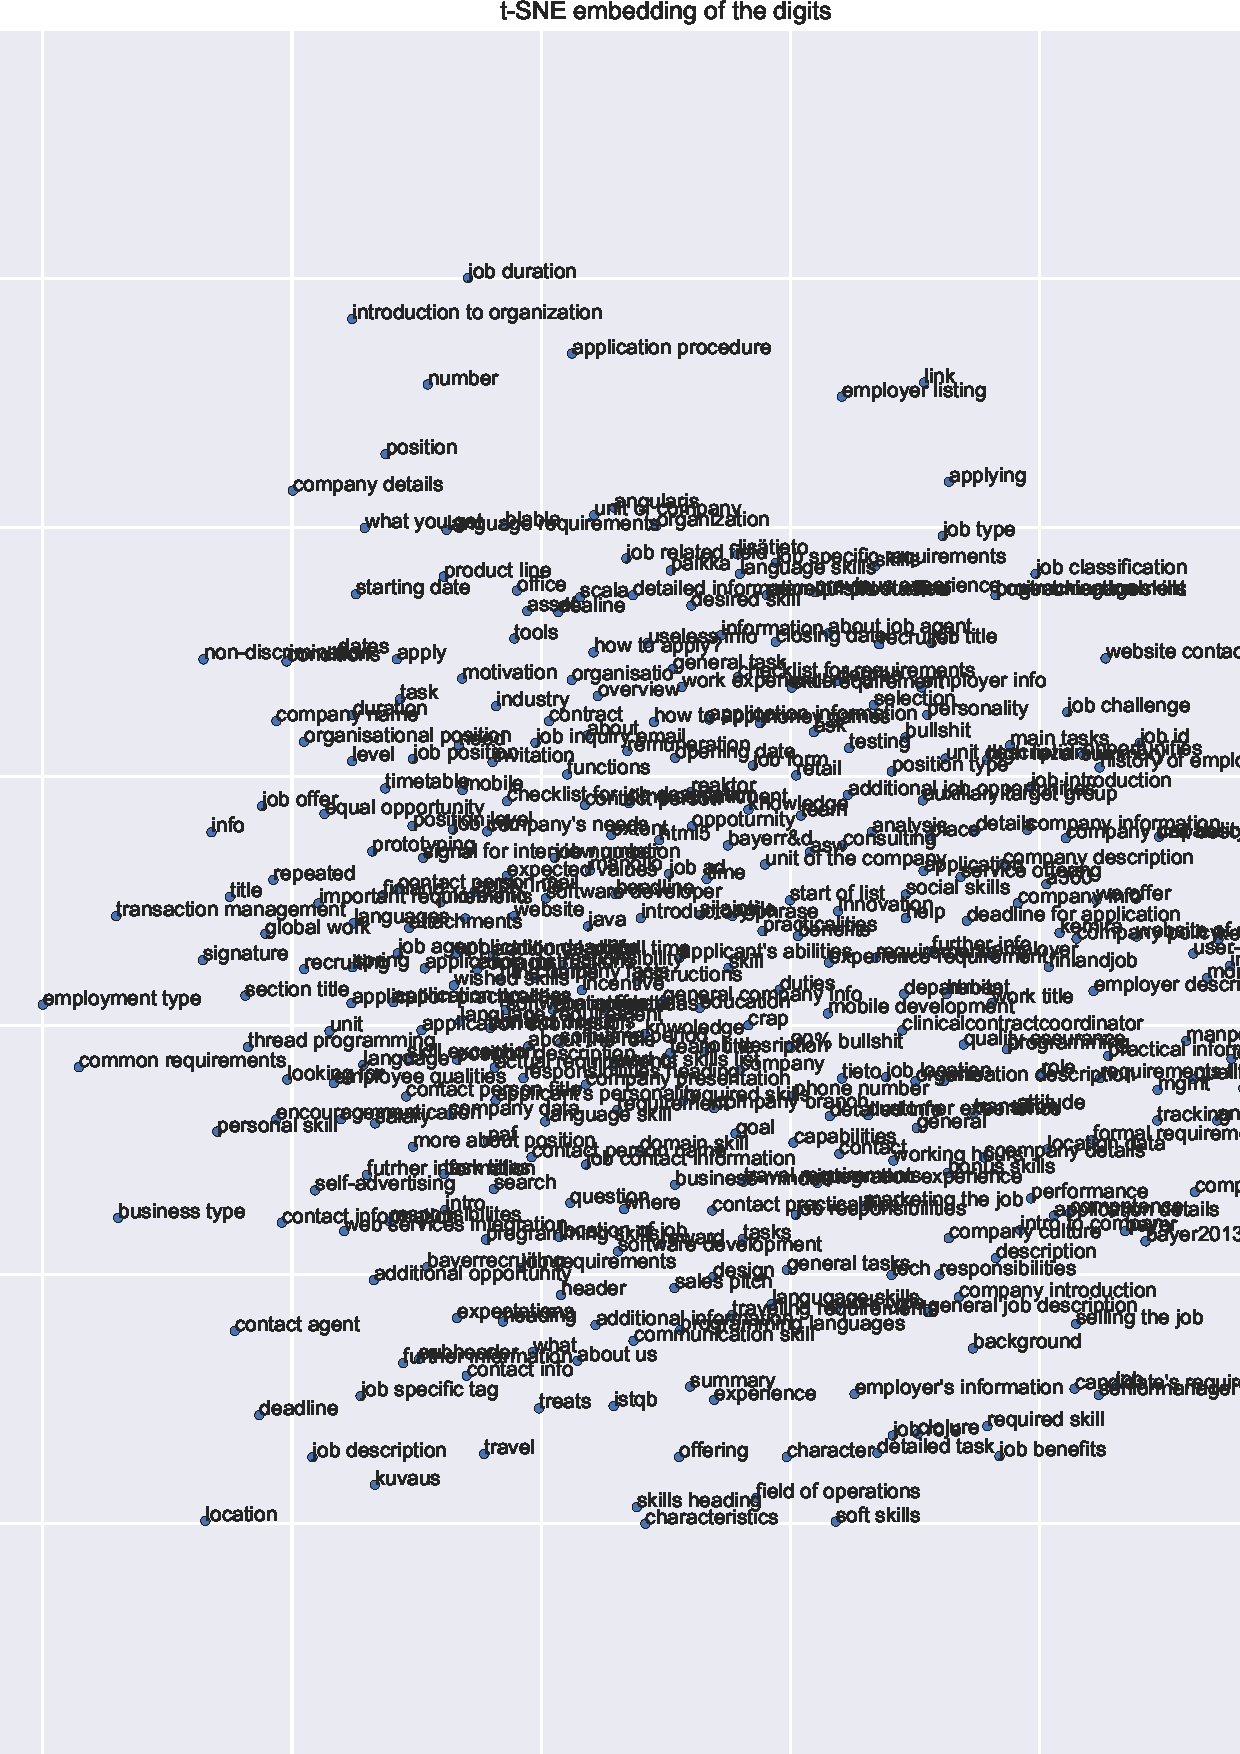
\includegraphics[width=\textwidth]{img/paragraph-data-tSNE.pdf}
    \caption{t-SNE Embedding}
  \label{fig:paragraph-data-tSNE}
\end{figure}

\begin{figure}[h]
    \centering
    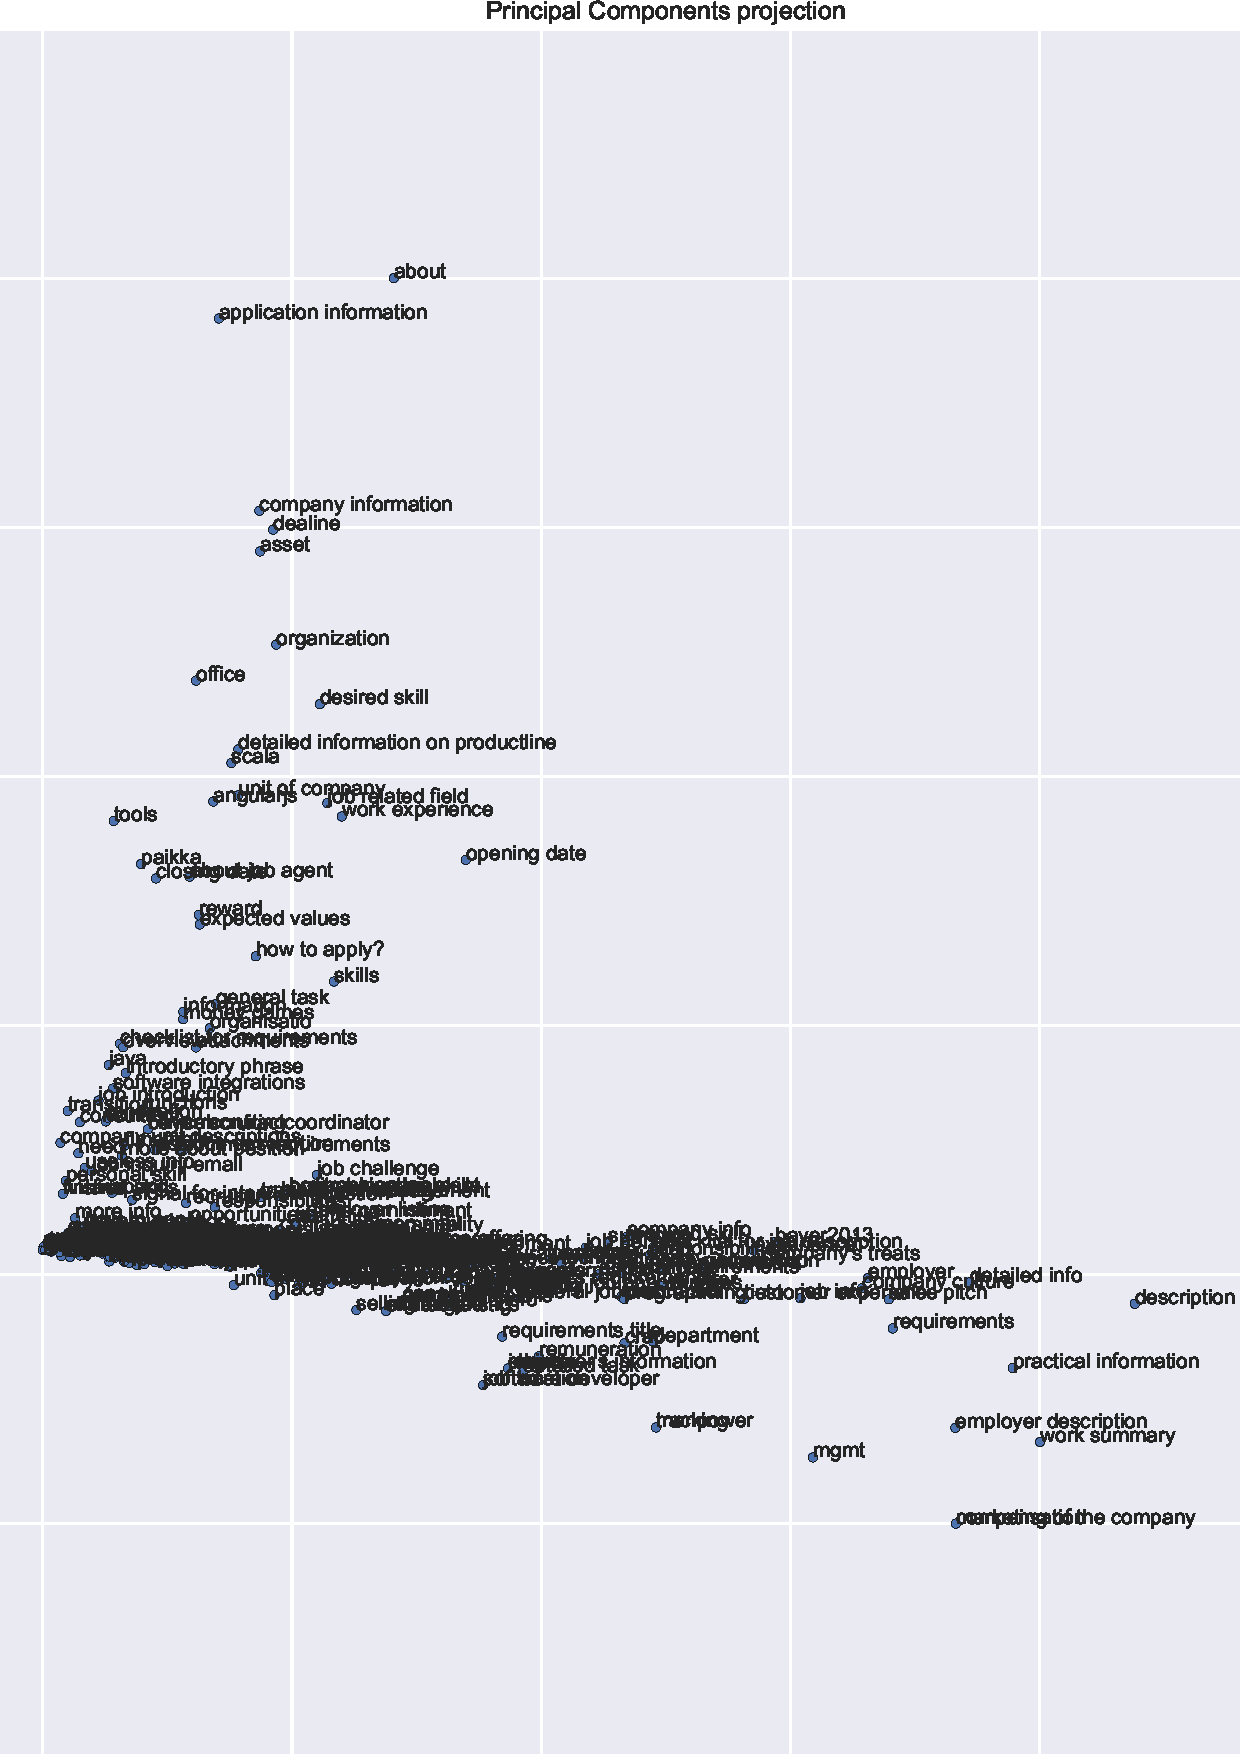
\includegraphics[width=\textwidth]{img/paragraph-data-principal-components-projection.pdf}
    \caption{Principal Components Projection}
  \label{fig:paragraph-data-principal-components-projection}
\end{figure}

\subsubsection{Crowdsourced Data Collection with Refined Research Problem}


\begin{figure}[h]
 % From http://localhost:8888/notebooks/thesis/experiments/vector-space-models/Vector%20Space%20Models.ipynb#Setup
    \centering
    \begin{subfigure}[b]{0.46\textwidth}
        \includegraphics[width=\textwidth]{img/sentence-data-judgement-confidence.pdf}
        \caption{Confidence}
      \label{fig:sentence-data-judgement-confidence}
    \end{subfigure}
    ~
    %add desired spacing between images, e. g. ~, \quad, \qquad, \hfill etc.
    %(or a blank line to force the subfigure onto a new line)
    \begin{subfigure}[b]{0.43\textwidth}
        \includegraphics[width=\textwidth]{img/sentence-data-judgement-confidence-cumulative.pdf}
        \caption{Cumulative Confidence}
        \label{fig:sentence-data-judgement-confidence-cumulative}
    \end{subfigure}
    \caption{Amount of label judgements versus label confidence of the sentence label data collected via crowdflower}
  \label{fig:sentence-data-judgements}
\end{figure}


\begin{figure}[h]
  % From http://localhost:8888/notebooks/thesis/experiments/vector-space-models/Vector%20Space%20Models.ipynb#Setup
    \centering
    \includegraphics[width=\textwidth]{img/sentence-data-label-dist.pdf}
    \caption{Distribution of labels in sentence data}
  \label{fig:sentence-data-label-dist}
\end{figure}

\clearpage

\section{Evaluation}
\label{sec:evaluation}

\todo{explain suervised classifiaction and binaty vs multi}

\subsection{Binary Classification}
\label{sub:binary-classification}

In binary or dichotomous case of classification we are given a single class $k$ and a set of labelled data points $\mathcal{D} = \{ (x_1, y_1), (x_2, y_2), \ldots, (x_n, y_n) \}$ where targets $y_i \in \{0, 1\}$ encode whether a data point $x_i$ belongs the class $c$ or not. The task is then to achieve correct classification of new data points without knowing the true label via a model function or predictor $f(\cdot)$.

To evaluate such a predictor it is useful to present the results in form of a contingency table as shown in table Table~\ref{table:contingency-table-2}, because it gives valuable insights about the performance of the prediction. The table shows the proportion of data points that belong to the class (RP) or not (RN) and were predicted correctly (TP) or incorrectly (FN), as well as the number of data samples that do not belong to the class (RN) and were falsely predicted to be in the class (FP) or correctly predicted to not be in the class (TN), and the same proportions for the positively (PP) and negatively (PN) predicted cases with respect to the true assignments to the data. N refers to the total amount of data points.

\begin{table}[h]
  \begin{center}
    \begin{tabular}{r | c c }
      & Real Positives (RP) & Real Negatives (RN) \\
      \hline
      Predicted Positives (PP) & True Positives (TP) & False Positives (FP) \\
      Predicted Negatives (PN) & False Negatives (FN) & True Negatives (TN) \\
    \end{tabular}
  \caption{Contingency table for binary classification}
  \label{table:contingency-table-2}
  \end{center}
\end{table}

An intuitive choice towards classification is to simply ask which data points were correctly classified to belong to the class or not. In terms of the contingency table above the ratio of $(\text{TP} + \text{FP}) / (\text{N})$, commonly referred to as the ``accuracy'' of the classifier.

This choice can give a good intuition and it does capture the effectiveness on both true positives as well as true negatives, but it is strongly influenced by bias of the true and predicted class distribution (known as prevalence RP/N and label bias) as pointed out by \cite{Powers:2011aa}. For example given a population of 900 positive and 100 negative examples, a predictor that simply always chooses a positive assignment can achieve accuracy of 90\% while it obviously is not a great predictor.

\subsubsection{Precision, Recall and F1 Score}
\label{subs:precision-recall-f1score}

In the field of Information Retrieval it is common practice to measure the effectiveness of a predictive system in terms of its precision and recall.
The precision of such system is \textquote{the proportion of retrieved material that is actually relevant} whereas the recall measures \textquote{proportion of relevant material actually retrieved in answer to a search request}~\cite{Rijsbergen:1979aa}. Formally these two measures are defined as:

\begin{equation}
    \text{Precision} = \frac{\text{TP}}{\text{TP} + \text{FP}}
\end{equation}
\begin{equation}
    \text{Recall} = \frac{\text{TP}}{\text{TP} + \text{FN}}
\end{equation}


As both, high precision and recall, are important for an robust information retrieval system they are typically combined into a single measure such as the F-measure, also referred to as F-score. The F-score is the weighted harmonic mean between precision and recall, derived from the measure of effectiveness proposed in~\cite{Rijsbergen:1979aa}. The most common form is the $F_1$ score  where precision and recall are assigned equal weight:
\begin{equation}
  \label{f1measure}
  F_1 = 2 \cdot \frac{\text{Precision} \cdot \text{Recall}}{\text{Precision} + \text{Recall}}
\end{equation}

The $F_1$ score has the advantage of its intuitive interpretability as both precision and recall are well understood measures and, analogous to recall, precision and accuracy, as it lives in the range $[0,1]$, giving a single number that can express the effectiveness of the system in terms of percentage.

The F1 score is widely used in the field of Machine Learning and Data Mining and thus it is an important measure to consider to compare results to outcomes of prior publications by others.
It is however important to point out that any version of the F-measure is a biased score as it \textquote{ignores TN which can vary freely without affecting the statistic}~\cite{Powers:2011aa}. This can affect the evaluation of a classifier when the class distribution is skewed (prevalence) or the classifier develops a bias towards certain classes (label bias), motivating the use of unbiased measures in these cases, such as the ones described next.

\subsubsection{Informedness, Markedness and Matthews Correlation Coefficient}
\label{subs:informedness-markedness-mcc}

\cite{Powers:2011aa} introduces unbiased analogue measures to Recall and Precision, called ``Informedness'' and ``Markedness'' respectively. As \cite{Powers:2011aa} lays out, \blockquote{Informedness quantifies how informed a predictor is for the specified condition, and specifies the probability that a prediction is informed in relation to the condition (versus chance).}:

\begin{equation}
  \begin{split}
  \text{Informedness} &= \text{Recall} + \text{Inverse Recall} \text{ – } 1 \\
  &= 1 - \text{Miss Rate} - \text{Fallout} \\
  &= 1 - \frac{\text{FN}}{ \text{RN}} - \frac{\text{FP}}{\text{RP}}
  \end{split}
\end{equation}

Further he defines:
\blockquote{Markedness quantifies how marked a condition is for the specified predictor, and specifies the probability that a condition is marked by the predictor (versus chance).}

\begin{equation}
  \begin{split}
  \text{Informedness} &= \text{Recall} + \text{Inverse Recall} \text{ – } 1 \\
  &= 1 - \text{Miss Rate} - \text{Fallout} \\
  &= 1 - \frac{\text{FN}}{ \text{RN}} - \frac{\text{FP}}{\text{RP}}
  \end{split}
\end{equation}

Based on Informedness and Markedness we can then see that \emph{Matthews Correlation Coefficient} $r_{G}$, first proposed by \cite{Matthews:1975aa}, is a score that balances these two measures:

\begin{equation}
  \begin{split}
  r_{G} &= \pm \sqrt{\text{Informedness} \cdot \text{Markedness}} \\
  &= \frac{(\text{TP} \cdot \text{TN} - \text{FP} \cdot \text{FN})}{(\text{TP} + \text{FN})(\text{FP} + \text{TN})(\text{TP} + \text{FP})(\text{FN} + \text{TN})}
\end{split}
\end{equation}

Matthews Correlation Coefficient can thus be used as unbiased alternative to the F-measure and offers a similar ease of interpretability as it ranges from -1 to 1, the former indicating a negative correlation or adverse estimation and the latter  indicating a perfect prediction, while a coefficient of 0 reflects chance.

\subsection{Multi-class classification}

Multi-class classification refers to a generalization of the binary case where we aim to predict for each datapoint $x_i$ one of $K$ labels for the classes at hand. The target space $\mathcal{Y}$ can be represented with each $y_i \in \{0,1\}^k$, known as \emph{one-hot encoding}, where each target is $c$-dimensional vector. Alternatively we can encode the targets as categorical variables $y_i \in {c_1, c_2, \ldots, c_k}$. The contingency table from the binary case can be extended as in table~\ref{table:contingency-table-k}, which is then commonly known as \emph{Confusion Matrix} or \emph{Error Matrix} \todo{citation for Confusion Matrix?}.

\begin{center}
  \begin{table}[h]
  \begin{tabular}{r | c c c c }
    & Real Class 1 & Real Class 2 & \ldots & Real Class $k$ \\
    \hline
    Predicted Class 1    & \ldots & \ldots & & \ldots \\
    Predicted Class 2    & \ldots & \ldots & & \ldots \\
    \ldots               & & & & \\
    Predicted Class $k$  & \ldots & \ldots & & \ldots \\
  \end{tabular}
  \caption{Contingency table for $k$ classes, also referred to as Confusion Matrix}
\label{table:contingency-table-k}
\end{table}
\end{center}

\subsubsection{Averaging for Multi-class Recall, Precision and F1-Score}

A way to evaluate


\subsubsection{Matthews Correlation Coefficient for K classes}

\subsubsection{Categorical Cross-entropy / Multi-class Log-loss}

\subsection{Multi-label classification}





\section{Statistical Language Modeling}
\label{sec:vector-space-models}


Thus each document document vector has the same dimensionality its dimensions can be used as features to be fed into most popular classification metho

\subsection{N-gram language models}
\label{subs:n-gram-language-models}

N-gram language models are based on co-occurrences of word or character sequences, so-called N-grams or $k$-shingles as they are referred to in the Data Mining literature~\cite[Chapter 3.2, p.~72]{Leskovec:2014aa}. Formally an N-gram is defined as a sequence of $n$ items, each of which consist of $n$ characters or words, effectively used to capture sub-sequences of text. Common choices are N-grams of size 1, 2 or 3 --- called \emph{unigrams}, \emph{bigrams} and ``trigrams'' respectively --- and the definition can be extended to using a window size $[\textit{w}_{\text{min}}, \textit{w}_{\text{max}}]$, employing all combinations of N-grams in this interval.

N-grams are usually used to create a vector-space model by representing each document in a dataset as a \textit{bag-of-words} or \textit{bag-of-N-grams} vector so that each dimension of the vector represents statistics about the corresponding N-gram. Specifically, a common way to compute the word count vectors for a document is the following:

\begin{equation}
  \text{TF}_{ij} = \frac{f_{ij}}{\max_k f_{kj}}
\end{equation}

Where $f_{ij}$ is \textquote{the \emph{frequency} (number of occurences) of a term (word) $i$ in document $j$} and $\text{TF}_{if}$ is the \emph{term frequency}, i.e.   \textquote{$f_{ij}$ normalized by dividing it by the maximum number of occurrences of any term [\ldots] in the same document}~\cite[Chapter 1.3.1, p.~8]{Leskovec:2014aa}.

As this approach has been studied for decades \todo{citation for first or review paper here?} there is quite an extensive amount of variants and thus hyper-parameters to tune. The most important ones will be explained in the following sections:

\paragraph{Words vs. Characters} The first choice when building an N-gram language model is to use characters or words as the atomic unit. In practically every case there are less characters than words in a dataset, but to capture expressive substrings usually larger N-gram window sizes or ranges have to be chosen, which leads to a combinatorial explosion. In case of word-based models on the other hand the maximal size of the feature space is the size of the vocabulary $\mathcal{V}$ in the case of unigrams or $V^k$ in case of $k$-grams.

\paragraph{Stop words} For creating N-gram models, so-called stop word lists are often used which are lists of frequent words that will be excluded as they do not carry much meaning~\cite[Chapter 1.3.1, p.~7]{Leskovec:2014aa}. The stop-word list used in these experiments is the standard list used for the Scikit-learn framework \cite{Pedregosa:2011aa} which is a list gathered by the University of Glasgow Information Retrieval group \footnote{\url{http://www.gla.ac.uk/schools/computing/research/researchoverview/informationretrieval/}. The full stop word list can be found at \url{http://ir.dcs.gla.ac.uk/resources/linguistic_utils/stop_words} and in the appendix in section \ref{sec:appendix-stopwords}.}.

\paragraph{N-gram range} The N-gram range, also known as window size or shingle size, refers to combinations of the atomic units of the model (words or characters) and defines an upper and lower limit for these combinations. For example a range of $[1,1]$ specifies a unigram model, $[2,2]$ a bigram model and $[1,2]$ a combination of both including all unigrams and all bigrams.
A larger range allows the model to capture an increasing amount of word order and thus context, but again leads to a combinatorial explosion in terms of feature space.

\paragraph{Vector size} The vector size imposes an upper limit to the vector size and therefor the number of N-grams that can be encoded in the feature space. Commonly this simply uses the words with the highest frequency to reduce the vector size from the full length --- the size of the vocabulary --- to the desired size.

\paragraph{TF.IDF weighting}

- TF.IDF vs simple wordcounts
- sublinear TF
- norm

- show T-SNE embeddings of doc2vec vectors

\todo{stemming}

Today N-gram models are still in wide use and considered as state of the art \textquote{not because there are no better techniques, but because those better techniques are computationally much more complex, and provide just marginal improvements}~\cite[p.~17]{Mikolov:2012aa}.

Notable shortcomings of this method are it's inability to capture word-order

\begin{itemize}
  \item vector space models
  \item bag of words
  \item \textquote{The most important weakness is that the number of possible n-grams increases exponentially with the length of the context, preventing these models to effectively capture longer context patterns. This is especially painful if large amounts of training data are available, as much of the patterns from the training data cannot be effectively represented by n-grams and cannot be thus discovered during training. The idea of using neural network based LMs is based on this observation, and tries to overcome the exponential increase of parameters by sharing parameters among similar events, no longer requiring exact match of the history H.}~\cite[p.~17]{Mikolov:2012aa}
\end{itemize}

\section{Classification Approaches}

\subsection{Discriminant Functions for Multi-class Classification}

A simple approach to multi-class classification is to pose the learning problem as a combination of binary classification problems as described in~\cite[Chapter 4.1.2, p.~182]{Bishop:2006aa}. This can be done by using $K$ separate classifiers, each of which predicts one of the classes against all $K-1$ other classes, which is known as the \textit{one-versus-the-rest} classification scheme. An alternative approach is to train $K (K - 1) / 2$ binary classifiers for each possible pair of classes, referred to as \textit{one-versus-one} classification.

These extensions though have major drawbacks as pointed out by~\cite[Chapter 5.2.2]{Duda:1973aa}. As illustrated by~\ref{fig:Bishop2006aa-p182-ch4-fig4-1} both of the classification schemes lead to ambiguous regions in the hypothesis space as their classification is undefined.

\begin{figure}[h]
    \centering
    \begin{subfigure}[b]{0.4\textwidth}
        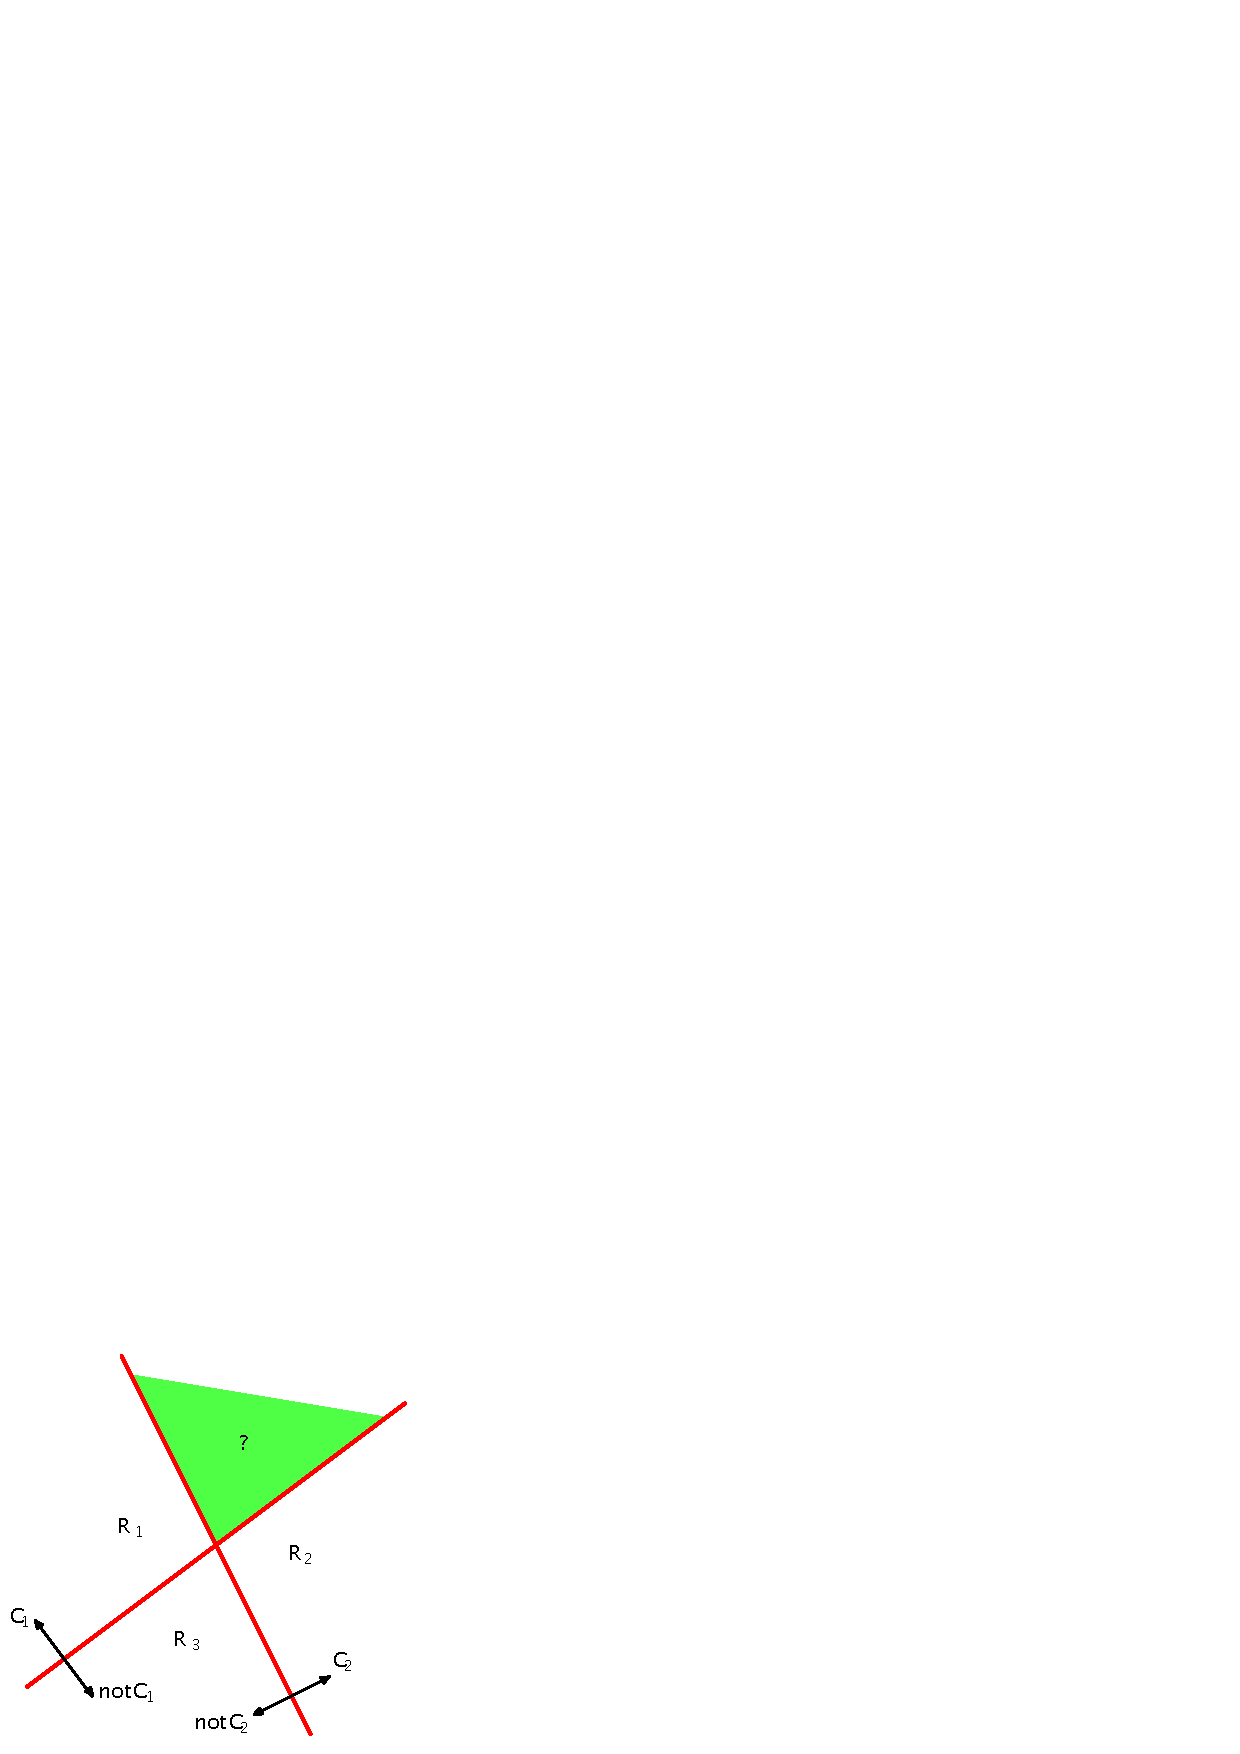
\includegraphics[width=\textwidth]{img/Bishop2006aa-p182-ch4-fig4-1-a.pdf}
        \caption{One-Vs-Rest classification scheme}
        \label{fig:Bishop2006aa-p182-ch4-fig4-1-a}
    \end{subfigure}
    ~ %add desired spacing between images, e. g. ~, \quad, \qquad, \hfill etc.
      %(or a blank line to force the subfigure onto a new line)
    \begin{subfigure}[b]{0.4\textwidth}
        \includegraphics[width=\textwidth]{img/Bishop2006aa-p182-ch4-fig4-1-b.pdf}
        \caption{One-Vs-One classification scheme}
        \label{fig:Bishop2006aa-p182-ch4-fig4-1-b}
    \end{subfigure}
    \caption{: Ambiguous regions in the hypothesis space (\cite{Bishop:2006aa} Chapter 4, Figure 4.1) }
    \label{fig:Bishop2006aa-p182-ch4-fig4-1}
\end{figure}

\cite{Bishop:2006aa}

% \subsection{Collecting Data}
%
% \begin{itemize}
%
% \item Document data extraction for crowdflower:
http://localhost:8888/notebooks/thesis/sandbox/crowdflower-data-collection/extract-data-crowdflower.ipynb
%
% \end{itemize}
%
% \subsubsection{Paragraph labels: Manual crowd-sourcing}
%
% \subsubsection{Sentence labels: Crowd-sourced collection via Crowdflower}
%
% \subsection{Feature extraction from Text Data}
%
% \subsubsection{N-grams}
%
% Relevant sources: \cite{Chen:1996aa}
%
% \subsubsection{Word2Vec}
%
% \subsection{Supervised Classification Methods}
%
% \subsection{Prediction Settings}
%
% \subsubsection{Multi-class multi-output prediction on paragraphs}
%
% \subsubsection{Multi-class single-output prediction on sentences}
